\documentclass[]{article}
\usepackage{lmodern}
\usepackage{amssymb,amsmath}
\usepackage{ifxetex,ifluatex}
\usepackage{fixltx2e} % provides \textsubscript
\ifnum 0\ifxetex 1\fi\ifluatex 1\fi=0 % if pdftex
  \usepackage[T1]{fontenc}
  \usepackage[utf8]{inputenc}
\else % if luatex or xelatex
  \ifxetex
    \usepackage{mathspec}
  \else
    \usepackage{fontspec}
  \fi
  \defaultfontfeatures{Ligatures=TeX,Scale=MatchLowercase}
\fi
% use upquote if available, for straight quotes in verbatim environments
\IfFileExists{upquote.sty}{\usepackage{upquote}}{}
% use microtype if available
\IfFileExists{microtype.sty}{%
\usepackage{microtype}
\UseMicrotypeSet[protrusion]{basicmath} % disable protrusion for tt fonts
}{}
\usepackage[margin=1in]{geometry}
\usepackage{hyperref}
\hypersetup{unicode=true,
            pdftitle={Statistical Inference: Exponential Distribution},
            pdfauthor={Sanjay Somraj},
            pdfborder={0 0 0},
            breaklinks=true}
\urlstyle{same}  % don't use monospace font for urls
\usepackage{color}
\usepackage{fancyvrb}
\newcommand{\VerbBar}{|}
\newcommand{\VERB}{\Verb[commandchars=\\\{\}]}
\DefineVerbatimEnvironment{Highlighting}{Verbatim}{commandchars=\\\{\}}
% Add ',fontsize=\small' for more characters per line
\usepackage{framed}
\definecolor{shadecolor}{RGB}{248,248,248}
\newenvironment{Shaded}{\begin{snugshade}}{\end{snugshade}}
\newcommand{\KeywordTok}[1]{\textcolor[rgb]{0.13,0.29,0.53}{\textbf{{#1}}}}
\newcommand{\DataTypeTok}[1]{\textcolor[rgb]{0.13,0.29,0.53}{{#1}}}
\newcommand{\DecValTok}[1]{\textcolor[rgb]{0.00,0.00,0.81}{{#1}}}
\newcommand{\BaseNTok}[1]{\textcolor[rgb]{0.00,0.00,0.81}{{#1}}}
\newcommand{\FloatTok}[1]{\textcolor[rgb]{0.00,0.00,0.81}{{#1}}}
\newcommand{\ConstantTok}[1]{\textcolor[rgb]{0.00,0.00,0.00}{{#1}}}
\newcommand{\CharTok}[1]{\textcolor[rgb]{0.31,0.60,0.02}{{#1}}}
\newcommand{\SpecialCharTok}[1]{\textcolor[rgb]{0.00,0.00,0.00}{{#1}}}
\newcommand{\StringTok}[1]{\textcolor[rgb]{0.31,0.60,0.02}{{#1}}}
\newcommand{\VerbatimStringTok}[1]{\textcolor[rgb]{0.31,0.60,0.02}{{#1}}}
\newcommand{\SpecialStringTok}[1]{\textcolor[rgb]{0.31,0.60,0.02}{{#1}}}
\newcommand{\ImportTok}[1]{{#1}}
\newcommand{\CommentTok}[1]{\textcolor[rgb]{0.56,0.35,0.01}{\textit{{#1}}}}
\newcommand{\DocumentationTok}[1]{\textcolor[rgb]{0.56,0.35,0.01}{\textbf{\textit{{#1}}}}}
\newcommand{\AnnotationTok}[1]{\textcolor[rgb]{0.56,0.35,0.01}{\textbf{\textit{{#1}}}}}
\newcommand{\CommentVarTok}[1]{\textcolor[rgb]{0.56,0.35,0.01}{\textbf{\textit{{#1}}}}}
\newcommand{\OtherTok}[1]{\textcolor[rgb]{0.56,0.35,0.01}{{#1}}}
\newcommand{\FunctionTok}[1]{\textcolor[rgb]{0.00,0.00,0.00}{{#1}}}
\newcommand{\VariableTok}[1]{\textcolor[rgb]{0.00,0.00,0.00}{{#1}}}
\newcommand{\ControlFlowTok}[1]{\textcolor[rgb]{0.13,0.29,0.53}{\textbf{{#1}}}}
\newcommand{\OperatorTok}[1]{\textcolor[rgb]{0.81,0.36,0.00}{\textbf{{#1}}}}
\newcommand{\BuiltInTok}[1]{{#1}}
\newcommand{\ExtensionTok}[1]{{#1}}
\newcommand{\PreprocessorTok}[1]{\textcolor[rgb]{0.56,0.35,0.01}{\textit{{#1}}}}
\newcommand{\AttributeTok}[1]{\textcolor[rgb]{0.77,0.63,0.00}{{#1}}}
\newcommand{\RegionMarkerTok}[1]{{#1}}
\newcommand{\InformationTok}[1]{\textcolor[rgb]{0.56,0.35,0.01}{\textbf{\textit{{#1}}}}}
\newcommand{\WarningTok}[1]{\textcolor[rgb]{0.56,0.35,0.01}{\textbf{\textit{{#1}}}}}
\newcommand{\AlertTok}[1]{\textcolor[rgb]{0.94,0.16,0.16}{{#1}}}
\newcommand{\ErrorTok}[1]{\textcolor[rgb]{0.64,0.00,0.00}{\textbf{{#1}}}}
\newcommand{\NormalTok}[1]{{#1}}
\usepackage{graphicx,grffile}
\makeatletter
\def\maxwidth{\ifdim\Gin@nat@width>\linewidth\linewidth\else\Gin@nat@width\fi}
\def\maxheight{\ifdim\Gin@nat@height>\textheight\textheight\else\Gin@nat@height\fi}
\makeatother
% Scale images if necessary, so that they will not overflow the page
% margins by default, and it is still possible to overwrite the defaults
% using explicit options in \includegraphics[width, height, ...]{}
\setkeys{Gin}{width=\maxwidth,height=\maxheight,keepaspectratio}
\IfFileExists{parskip.sty}{%
\usepackage{parskip}
}{% else
\setlength{\parindent}{0pt}
\setlength{\parskip}{6pt plus 2pt minus 1pt}
}
\setlength{\emergencystretch}{3em}  % prevent overfull lines
\providecommand{\tightlist}{%
  \setlength{\itemsep}{0pt}\setlength{\parskip}{0pt}}
\setcounter{secnumdepth}{0}
% Redefines (sub)paragraphs to behave more like sections
\ifx\paragraph\undefined\else
\let\oldparagraph\paragraph
\renewcommand{\paragraph}[1]{\oldparagraph{#1}\mbox{}}
\fi
\ifx\subparagraph\undefined\else
\let\oldsubparagraph\subparagraph
\renewcommand{\subparagraph}[1]{\oldsubparagraph{#1}\mbox{}}
\fi

%%% Use protect on footnotes to avoid problems with footnotes in titles
\let\rmarkdownfootnote\footnote%
\def\footnote{\protect\rmarkdownfootnote}

%%% Change title format to be more compact
\usepackage{titling}

% Create subtitle command for use in maketitle
\newcommand{\subtitle}[1]{
  \posttitle{
    \begin{center}\large#1\end{center}
    }
}

\setlength{\droptitle}{-2em}
  \title{Statistical Inference: Exponential Distribution}
  \pretitle{\vspace{\droptitle}\centering\huge}
  \posttitle{\par}
  \author{Sanjay Somraj}
  \preauthor{\centering\large\emph}
  \postauthor{\par}
  \predate{\centering\large\emph}
  \postdate{\par}
  \date{March 22, 2017}


\begin{document}
\maketitle

\section{Statistical Inference Course Project - PART
1}\label{statistical-inference-course-project---part-1}

\subsection{Overview}\label{overview}

1 This project investigates the exponential distribution in R and
compare it with the Central Limit Theorem.\\
2 This project will investigate the distribution of averages of 40
exponentials over 1000 test simulations.\\
3 The Rate parameter, lambda = 0.2 for all of the simulations.\\
4 The exponential distribution can be simulated in R with rexp(n,
lambda).\\
5 The mean of exponential distribution is 1/lambda and the standard
deviation is also 1/lambda.

\subsection{Load libraries for data processing and
plotting}\label{load-libraries-for-data-processing-and-plotting}

\begin{Shaded}
\begin{Highlighting}[]
\KeywordTok{library}\NormalTok{(ggplot2)}
\CommentTok{# INITIALIZE CONSTANTS}
     \CommentTok{# LAMBDA for rexp}
          \NormalTok{lambda <-}\StringTok{ }\FloatTok{0.2}
     \CommentTok{# Number of EXPONENTIALS}
          \NormalTok{n <-}\StringTok{ }\DecValTok{40}
     \CommentTok{# Number of TEST SIMULATIONS}
          \NormalTok{numberOfSimulations <-}\StringTok{ }\DecValTok{1000}
     \CommentTok{# set the SEED for reproducability}
          \KeywordTok{set.seed}\NormalTok{(}\DecValTok{1000}\NormalTok{)}

\CommentTok{# EXECUTE TEST PRODUCING 40 X 1000 MATRIX}
\NormalTok{exponentialDistributions <-}\StringTok{ }
\StringTok{     }\KeywordTok{matrix}\NormalTok{(}\DataTypeTok{data=}\KeywordTok{rexp}\NormalTok{(n *}\StringTok{ }\NormalTok{numberOfSimulations, lambda), }
            \DataTypeTok{nrow=}\NormalTok{numberOfSimulations)}

\NormalTok{exponentialDistributionMeans <-}\StringTok{ }
\StringTok{     }\KeywordTok{data.frame}\NormalTok{(}\DataTypeTok{means=}\KeywordTok{apply}\NormalTok{(exponentialDistributions, }\DecValTok{1}\NormalTok{, mean))}

\NormalTok{minExpValue <-}\StringTok{ }\KeywordTok{min}\NormalTok{(exponentialDistributionMeans$means)}
\NormalTok{maxExpValue <-}\StringTok{ }\KeywordTok{max}\NormalTok{(exponentialDistributionMeans$means)}

\CommentTok{# PLOT THE DISTRIBUTION MEANS}
\KeywordTok{ggplot}\NormalTok{(}\DataTypeTok{data =} \NormalTok{exponentialDistributionMeans, }
       \KeywordTok{aes}\NormalTok{(}\DataTypeTok{x =} \NormalTok{means)) +}\StringTok{ }
\StringTok{     }\KeywordTok{geom_histogram}\NormalTok{(}\DataTypeTok{col=}\StringTok{"red"}\NormalTok{, }\DataTypeTok{fill =} \StringTok{"orange"}\NormalTok{, }\DataTypeTok{binwidth =} \FloatTok{0.1}\NormalTok{)+}
\StringTok{     }\KeywordTok{labs}\NormalTok{(}\DataTypeTok{title=}\StringTok{"Histogram of Distribution of Means"}\NormalTok{, }
          \DataTypeTok{x =} \StringTok{"Mean"}\NormalTok{, }\DataTypeTok{y =} \StringTok{"Frequency"}\NormalTok{) +}\StringTok{ }
\StringTok{     }\KeywordTok{scale_x_continuous}\NormalTok{(}\DataTypeTok{breaks=}\KeywordTok{seq}\NormalTok{(minExpValue,maxExpValue,}\DataTypeTok{by=}\FloatTok{0.5}\NormalTok{))}
\end{Highlighting}
\end{Shaded}

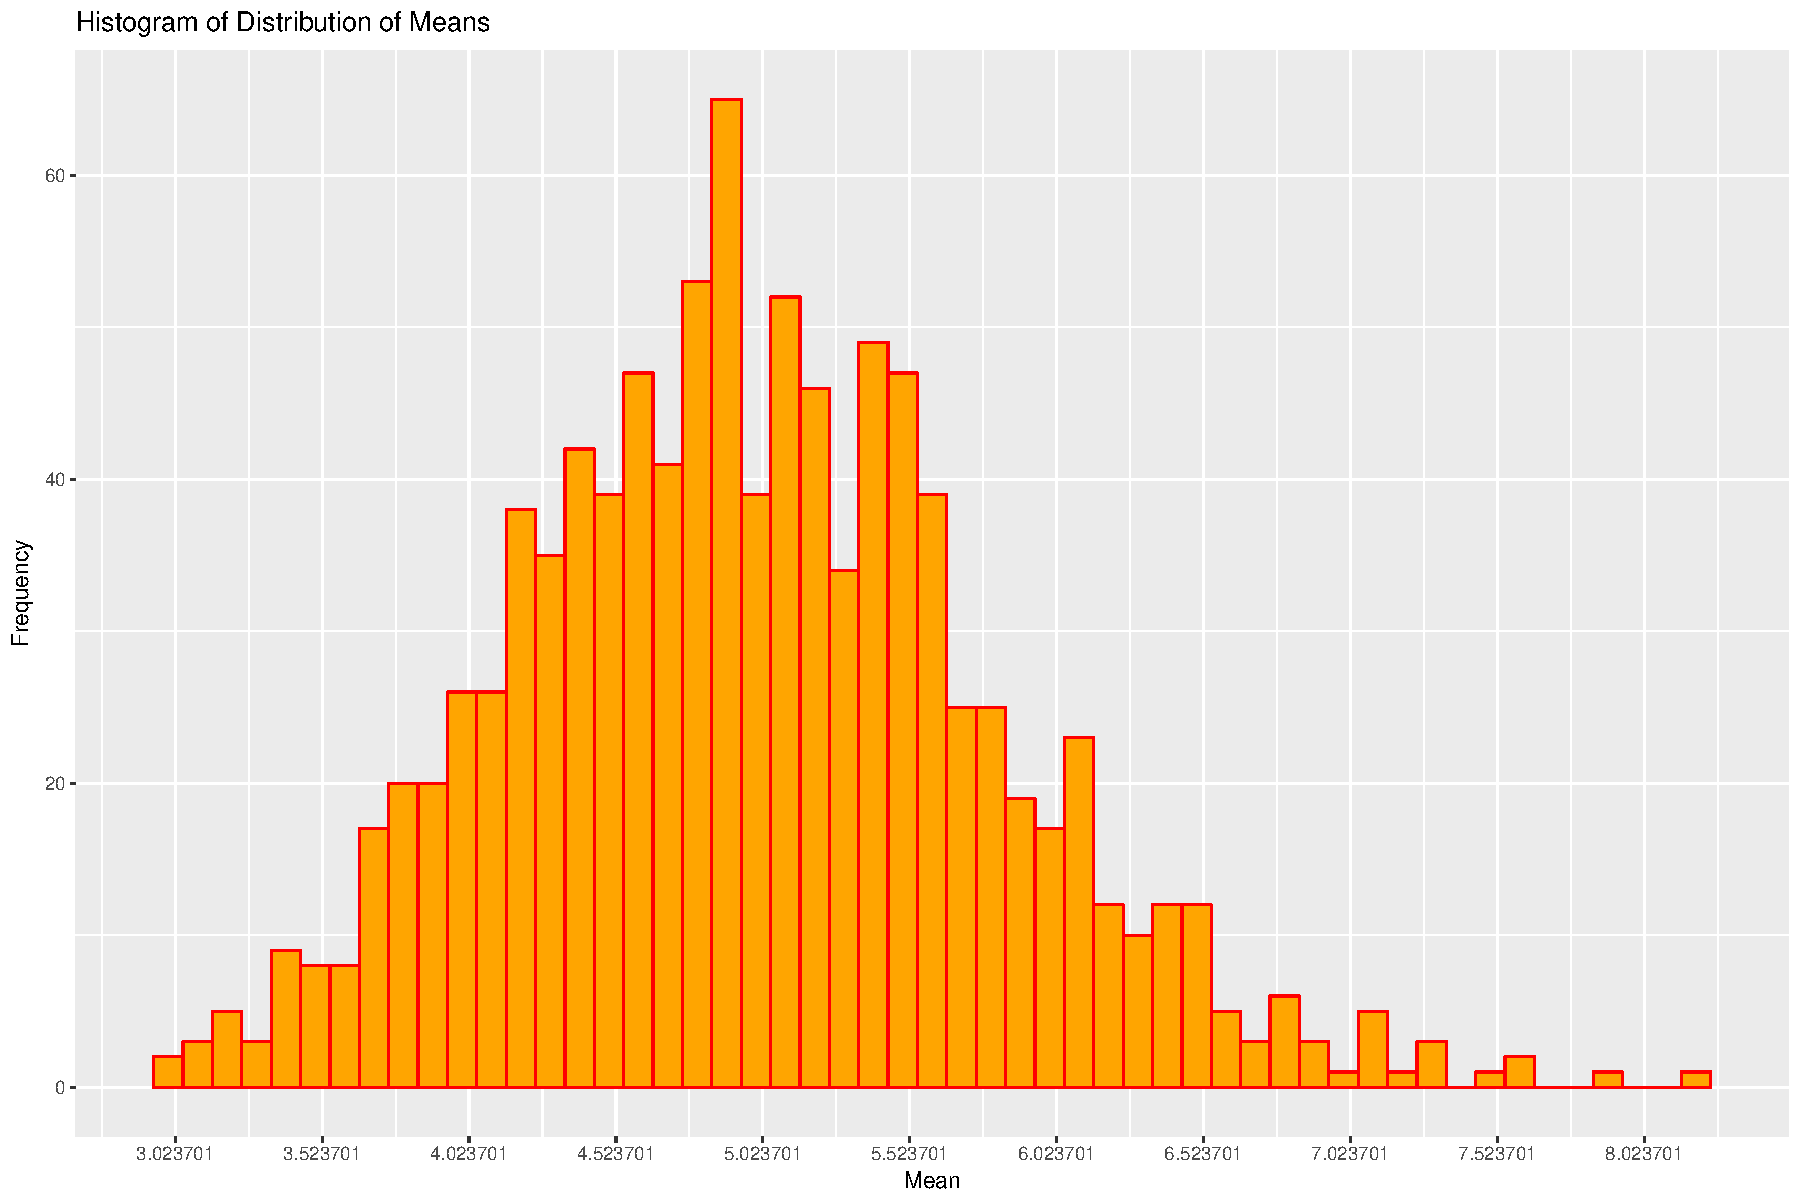
\includegraphics{Statistical_Inference_Project_1_files/figure-latex/unnamed-chunk-1-1.pdf}

\subsection{Sample Mean versus Theoretical
Mean}\label{sample-mean-versus-theoretical-mean}

First, let us compute the mean of sample means of the 1000 simulations
of 40 randomly sampled exponential distributions. We will compute
Theoretical Mean is the 1/lambda i.e.

\begin{Shaded}
\begin{Highlighting}[]
\NormalTok{sampleMean <-}\StringTok{ }\KeywordTok{mean}\NormalTok{(exponentialDistributionMeans$means)}
\NormalTok{theoryMean <-}\StringTok{ }\DecValTok{1}\NormalTok{/lambda}
\end{Highlighting}
\end{Shaded}

\textbf{Theoretical Mean:} 5\\
\textbf{Sample Mean:} 4.9869634

\textbf{We can see that SAMPLE MEAN (4.987) AND THEORETICAL MEAN (5) are
very close.}

\subsection{Sample Variance versus Theoretical
Variance}\label{sample-variance-versus-theoretical-variance}

Theoretical \textbf{STANDARD DEVIATION} is computed as mu/square-root(n)
i.e 1/lambda/sqrt(n)\\
And the \textbf{VARIANCE} is Square(Standard Deviation)

\begin{Shaded}
\begin{Highlighting}[]
\NormalTok{stdDev <-}\StringTok{ }\NormalTok{theoryMean/}\KeywordTok{sqrt}\NormalTok{(}\DecValTok{40}\NormalTok{)}
\NormalTok{varnc <-}\StringTok{ }\NormalTok{stdDev^}\DecValTok{2}

\NormalTok{sampleStdDev <-}\StringTok{ }\KeywordTok{sd}\NormalTok{(exponentialDistributionMeans$means)}
\NormalTok{sampleVarnc <-}\StringTok{ }\KeywordTok{var}\NormalTok{(exponentialDistributionMeans$means)}
\end{Highlighting}
\end{Shaded}

\begin{itemize}
\tightlist
\item
  \textbf{Theoretical Variance:} 0.625 \textbf{Sample Variance:}
  0.6583551\\
  \textbf{We observe that the Sample Variance is very close to
  Theoretical Variance.}
\end{itemize}

\subsection{Distribution}\label{distribution}

The plot shows the normal distribution and sample data distribution.

\begin{Shaded}
\begin{Highlighting}[]
\KeywordTok{ggplot}\NormalTok{(}\DataTypeTok{data =} \NormalTok{exponentialDistributionMeans, }\KeywordTok{aes}\NormalTok{(}\DataTypeTok{x =} \NormalTok{means)) +}\StringTok{ }
\StringTok{     }\KeywordTok{geom_density}\NormalTok{(}\DataTypeTok{colour=}\StringTok{"blue"}\NormalTok{, }\DataTypeTok{fill=}\StringTok{"blue"}\NormalTok{, }\DataTypeTok{alpha=}\FloatTok{0.1}\NormalTok{, }\DataTypeTok{size=}\DecValTok{1}\NormalTok{) +}
\StringTok{     }\KeywordTok{stat_function}\NormalTok{(}\DataTypeTok{fun =} \NormalTok{dnorm, }\DataTypeTok{args =} \KeywordTok{list}\NormalTok{(}\DataTypeTok{mean =} \NormalTok{theoryMean, }\DataTypeTok{sd =} \NormalTok{stdDev), }
                   \DataTypeTok{colour =} \StringTok{"red"}\NormalTok{, }\DataTypeTok{size=}\DecValTok{1}\NormalTok{) +}\StringTok{ }
\StringTok{     }\KeywordTok{scale_x_continuous}\NormalTok{(}\DataTypeTok{breaks=}\KeywordTok{seq}\NormalTok{(theoryMean}\DecValTok{-3}\NormalTok{, theoryMean}\DecValTok{+3}\NormalTok{,}\FloatTok{0.5}\NormalTok{),}
                        \DataTypeTok{limits=}\KeywordTok{c}\NormalTok{(theoryMean}\DecValTok{-3}\NormalTok{,theoryMean}\DecValTok{+3}\NormalTok{))+}
\StringTok{     }\KeywordTok{xlab}\NormalTok{(}\StringTok{'Sample Mean(BLUE) & Theoretical Mean(RED)'}\NormalTok{) +}\StringTok{ }\KeywordTok{ylab}\NormalTok{(}\StringTok{'Density'}\NormalTok{) +}
\StringTok{     }\KeywordTok{ggtitle}\NormalTok{(}\StringTok{'Sample distribution Vs Theoretical distribution'}\NormalTok{)}
\end{Highlighting}
\end{Shaded}

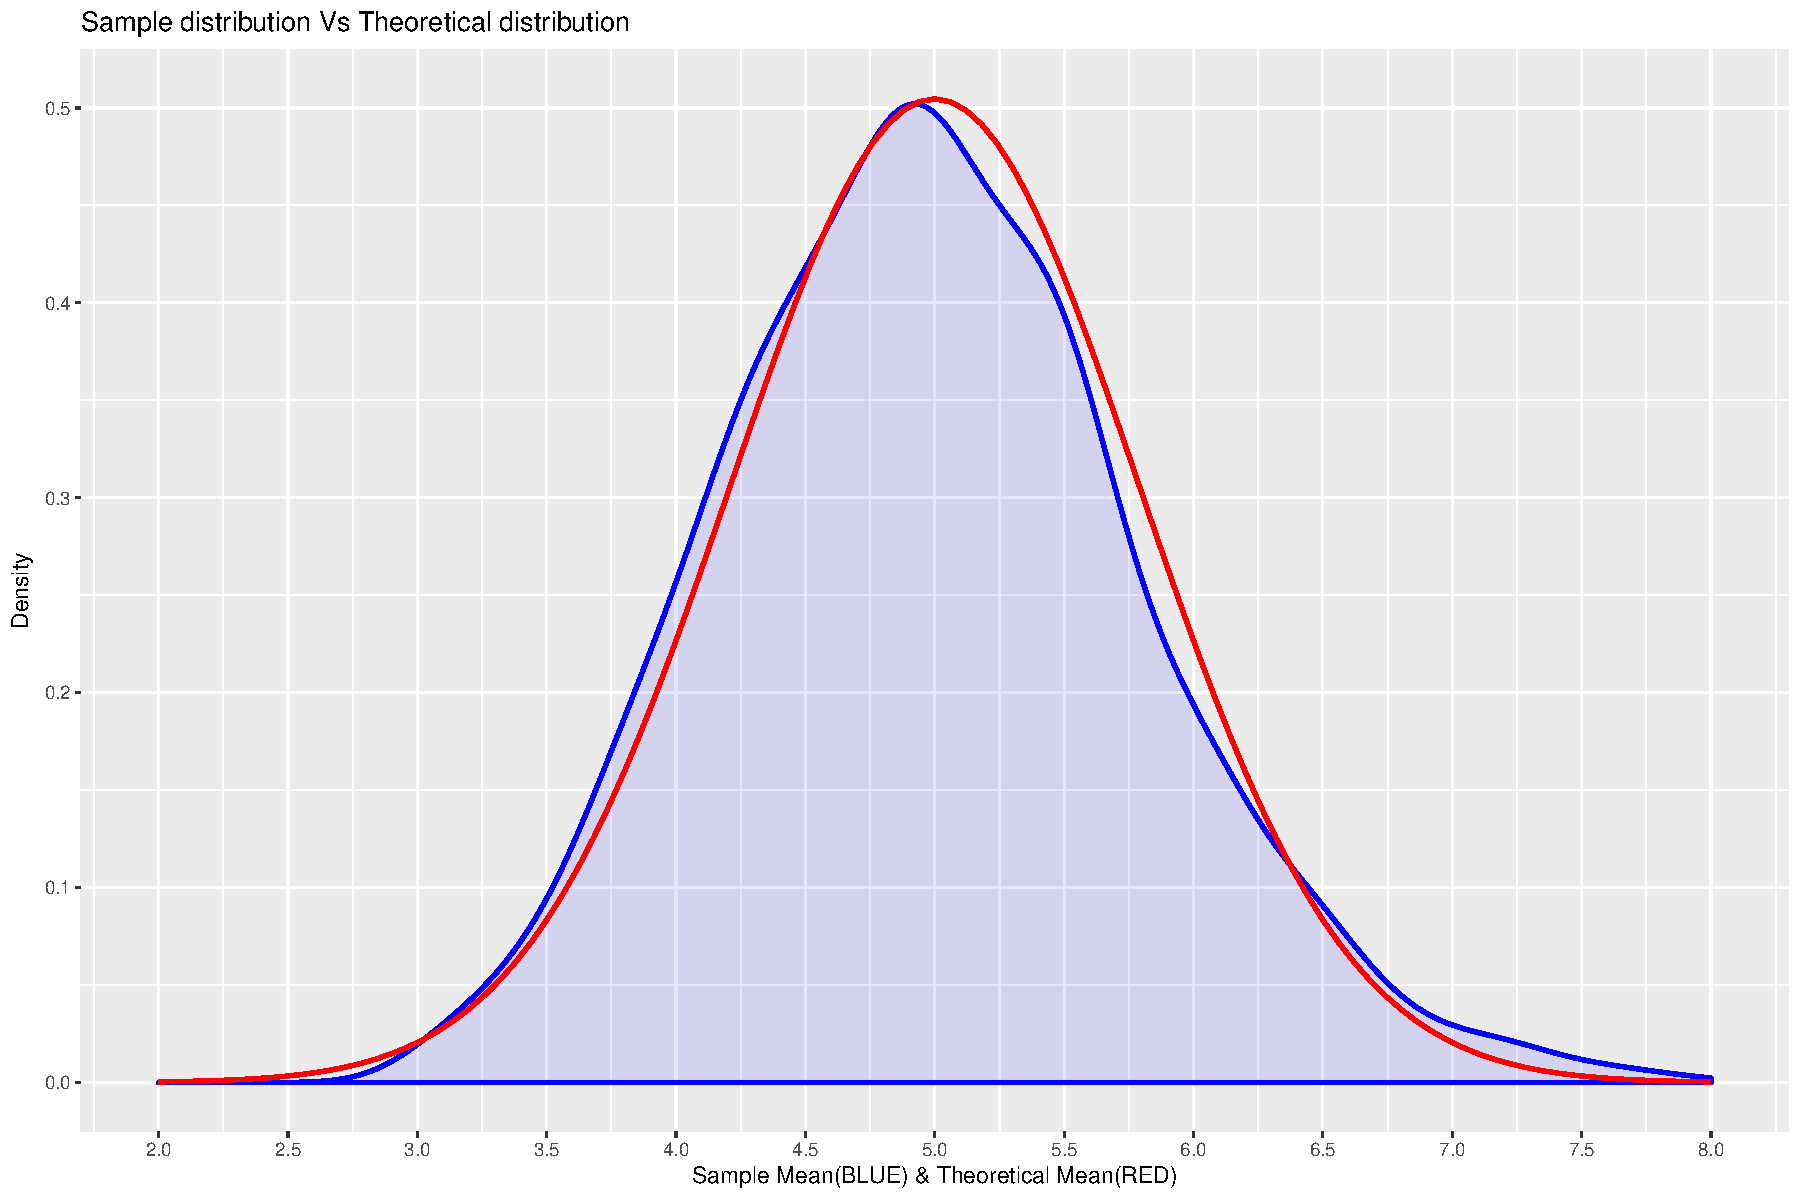
\includegraphics{Statistical_Inference_Project_1_files/figure-latex/unnamed-chunk-4-1.pdf}

\subsection{Summary}\label{summary}

For the given values of LAMBDA, N and the 1000 simulations, we observe
that the computed Sample Mean, Variance and Standard Deviation are very
close to respective Theoretical values.

The distribution of the sample and theoretical values are overlayed on
each other to help us with a clear view on the extent of overlap. The
RED line represents the Normal distribution while the BLUE line denotes
the sample data distribution. The calculated distribution of means of
random sampled exponential data overlaps with the normal distribution.


\end{document}
